\begin{center}
\Huge
	Komplekse tal som punkter.
\end{center}
\section*{Punktrepræsentation}
\stepcounter{section}

Et komplekst tal $z\in \mathbb{C}$ består som bekendt af en realdel Re$(z)$ og en imaginærdel Im$(z)$. Vi kan derfor vælge at repræsentere tallet $z$ som et punkt $(\textnormal{Re}(z), \textnormal{Im}(z))$. Dette koordinatsystem kaldes ofte det \textit{komplekse plan}, hvor $x$-aksen repræsenterer realdelen af tallet, og $y$-aksen repræsenterer imaginærdelen af tallet. Dette er vist på Figur \ref{fig:kompleksplan}.
\begin{figure}[H]
	\centering
	\begin{tikzpicture}
	\begin{axis}[
	axis lines = center, 
	ticks = none, 
	xmin = -2, xmax = 7, 
	ymin = -2, ymax = 6,
	xlabel = {Re},
	ylabel = {Im}
	]
		\filldraw[color = SeaGreen] (axis cs: 4,3) circle (2pt);
		\draw[dashed, color = SeaGreen, thick] (axis cs: 4,0) -- (axis cs: 4,3);
		\draw[dashed, color = SeaGreen, thick] (axis cs: 0,3) -- (axis cs: 4,3);
		\node[color = SeaGreen, anchor = south west] at (axis cs: 4,3) {$z$};
		\node[color = SeaGreen, anchor = north] at (axis cs: 4,0) {$\textnormal{Re}(z)$};
		\node[color = SeaGreen, anchor = east] at (axis cs: 0,3) {$\textnormal{Im}(z)$}; 
	\end{axis}	
	\end{tikzpicture}
	\caption{Repræsentation af et komplekst tal i det komplekse plan.}
	\label{fig:kompleksplan}
\end{figure}
Vi kan også betragte et eksempel.
\begin{exa}
	Vi ønsker at repræsentere de komplekse tal 
	$$z_1 = 2 + 4i$$ og 
	$$z_2 = 3 - 2i $$ i det komplekse plan. Vi tegner dem i
	et koordinatsystem på Figur \ref{fig:exa}.
	\begin{figure}[H]
		\centering
		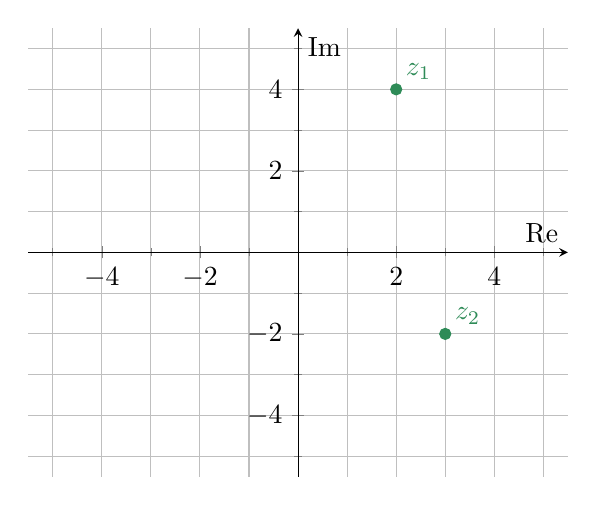
\begin{tikzpicture}
	\begin{axis}[
	axis lines = center, 
	xtick = {-8,-6,...,6,8},
	ytick = {-8,-6,...,6,8},
	grid = both, 
	minor tick num = 1,
	xmin = -5.5, xmax = 5.5, 
	ymin = -5.5, ymax = 5.5,
	xlabel = {Re},
	ylabel = {Im}
	]
		\filldraw[color = SeaGreen] (axis cs: 2,4) circle (2pt) node[anchor = south west] {$z_1$};
		\filldraw[color = SeaGreen] (axis cs: 3,-2) circle (2pt) node[anchor = south west] {$z_2$};
	\end{axis}	
	\end{tikzpicture}
	\caption{To komplekse tal $z_1$ og $z_2$ repræsenteret som punkter i det komplekse plan.}
	\label{fig:exa}
	\end{figure}
\end{exa}
For et komplekst tal kan det være meningsfuldt også at have en absolutværdi. Denne kaldes ofte \textit{modulus} og 
defineres på følgende vis.
\begin{defn}[Modulus]
	For et komplekst tal $z = a + bi$ defineres \textit{modulus} af $z$ som
	\begin{align*}
		|z| = \sqrt{a^2 + b^2}.
	\end{align*}
\end{defn}
Den geometriske fortolkning af modulus er afstanden fra origo til punktrepræsentationen af $z$ i det komplekse plan. Dette kan ses på Figur \ref{fig:modulus}.
\begin{figure}[H]
	\centering
	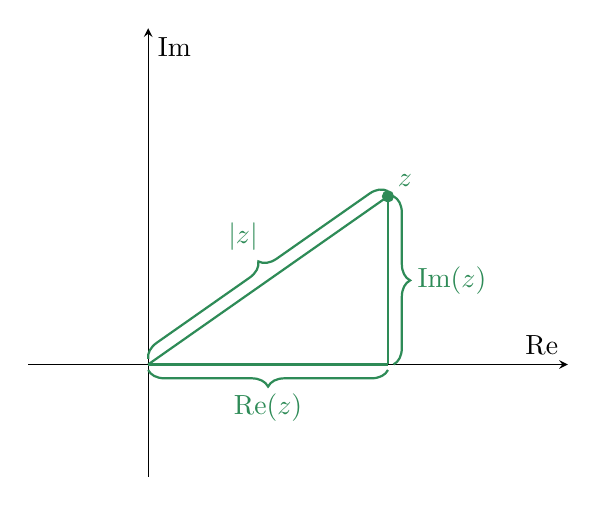
\begin{tikzpicture}
	\begin{axis}[
	axis lines = center, 
	ticks = none, 
	xmin = -2, xmax = 7, 
	ymin = -2, ymax = 6,
	xlabel = {Re},
	ylabel = {Im}
	]
		\filldraw[color = SeaGreen] (axis cs: 4,3) circle (2pt);
		\draw[color = SeaGreen, thick] (axis cs: 0,0) -- (axis cs: 4,0);
		\draw[color = SeaGreen, thick] (axis cs: 4,0) -- (axis cs: 4,3);
		\draw[color = SeaGreen, thick] (axis cs: 0,0) -- (axis cs: 4,3);
		\node[color = SeaGreen, anchor = south west] at (axis cs: 4,3) {$z$};
		\draw[decorate, decoration = {brace, amplitude = 6pt, mirror}, color = SeaGreen, yshift = -2pt, thick]
		(axis cs: 0,0) -- (axis cs: 4,0) node[midway, anchor = north, yshift = -5pt] {Re$(z)$};
		\draw[decorate, decoration = {brace, amplitude = 6pt, mirror}, color = SeaGreen, xshift = 2pt, thick]
		(axis cs: 4,0) -- (axis cs: 4,3) node[midway, anchor = west, xshift = 5pt] {Im$(z)$}; 
		\draw[decorate, decoration = {brace, amplitude = 6pt}, color = SeaGreen, yshift = 2pt, thick]
		(axis cs: 0,0) -- (axis cs: 4,3) node[midway, anchor = south east, yshift = 5pt] {$|z|$};
	\end{axis}	
	\end{tikzpicture}
	\caption{Modulus af et komplekst tal}
	\label{fig:modulus}
\end{figure}
Vi kan se, at vi har en retvinklet trekant på Figur \ref{fig:modulus}. Pythagoras' sætning fortæller os, at 
\begin{align*}
	a^2 + b^2 = c^2
\end{align*}
hvor $a$ og $b$ er kateter samt $c$ er hypotenusen i en retvinklet trekant. For et punkt $z\in \mathbb{C}$ har vi for kateterne, at 
\begin{align*}
	\textnormal{Re}(z)^2 + \textnormal{Im}(z)^2 = c^2 \
	 \Leftrightarrow \ c = \sqrt{\textnormal{Re}(z)^2 + \textnormal{Im}(z)^2} = |z|,
\end{align*}
og derfor tilsvarer modulus netop afstanden fra origo til punktet i det komplekse plan. 

\begin{exa}
	Vi ønsker at bestemme modulus for det komplekse tal $z_1 = -4 + 3i$. Vi indsætter i formlen og får
	\begin{align*}
		|z_1| = \sqrt{(-4)^2 + 3^2} = \sqrt{16+9} = \sqrt{25} = 5,
	\end{align*}
	og afstanden fra origo til $z_1$ i det komplekse plan er derfor 5.
	Vi kan tilsvarende bestemme modulus for $z_2 = 5 - 7i$. Dette giver os
	\begin{align*}
		|z_2| = \sqrt{5^2 + (-7)^2} = \sqrt{25+49} = \sqrt{74}.
	\end{align*}
\end{exa}

\newpage
\subsection*{Opgave 1}
\begin{enumerate}[label=\roman*)]
	\item Opskriv følgende komplekse tal på formen $z = a + bi$. 
	\item Bestem $z_1 + z_3$ og $z_6 - z_2$
	\item Bestem $z_4z_5$ og $z_{10}z_7$
	\item Bestem $\frac{z_8}{z_9}$ og $\frac{z_4}{z_6-z_2}$
\end{enumerate}

\begin{center}
	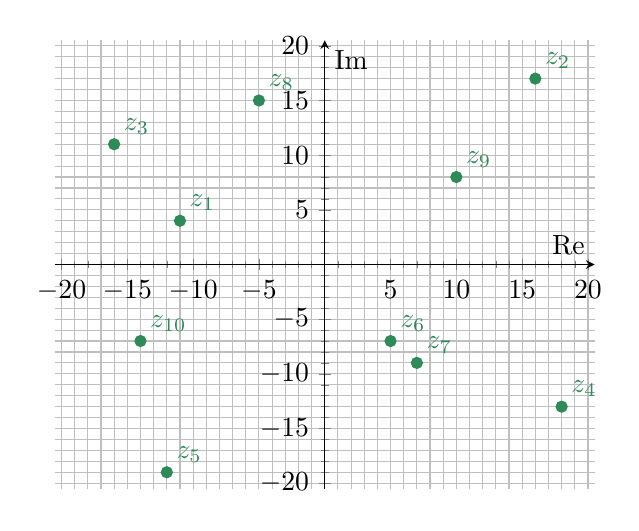
\begin{tikzpicture}
	\begin{axis}[
	axis lines = center, 
	xtick = {-20,-15,...,15,20},
	ytick = {-20,-15,...,15,20},
	grid = both, 
	minor tick num = 4,
	xmin = -20.5, xmax = 20.5, 
	ymin = -20.5, ymax = 20.5,
	xlabel = {Re},
	ylabel = {Im}
	]
		\filldraw[color = SeaGreen] (axis cs: -11,4) circle (2pt) node[anchor = south west] {$z_1$};
		\filldraw[color = SeaGreen] (axis cs: 16,17) circle (2pt) node[anchor = south west] {$z_2$};
		\filldraw[color = SeaGreen] (axis cs: -16,11) circle (2pt) node[anchor = south west] {$z_3$};
		\filldraw[color = SeaGreen] (axis cs: 18,-13) circle (2pt) node[anchor = south west] {$z_4$};
		\filldraw[color = SeaGreen] (axis cs: -12,-19) circle (2pt) node[anchor = south west] {$z_5$};
		\filldraw[color = SeaGreen] (axis cs: 5,-7) circle (2pt) node[anchor = south west] {$z_6$};
		\filldraw[color = SeaGreen] (axis cs: 7,-9) circle (2pt) node[anchor = south west] {$z_7$};
		\filldraw[color = SeaGreen] (axis cs: -5,15) circle (2pt) node[anchor = south west] {$z_8$};
		\filldraw[color = SeaGreen] (axis cs: 10,8) circle (2pt) node[anchor = south west] {$z_9$};
		\filldraw[color = SeaGreen] (axis cs: -14,-7) circle (2pt) node[anchor = south west] {$z_{10}$};
	\end{axis}	
	\end{tikzpicture}
\end{center}

\subsection*{Opgave 2}
Bestem modulus for følgende komplekse tal
\begin{center}
	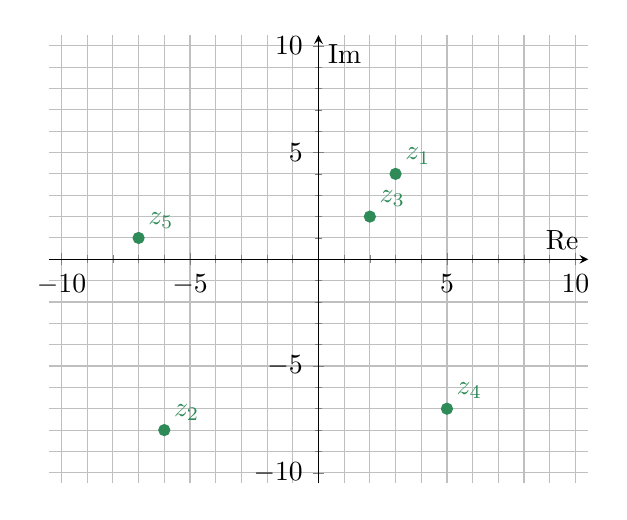
\begin{tikzpicture}
	\begin{axis}[
	axis lines = center, 
	xtick = {-20,-15,...,15,20},
	ytick = {-20,-15,...,15,20},
	grid = both, 
	minor tick num = 4,
	xmin = -10.5, xmax = 10.5, 
	ymin = -10.5, ymax = 10.5,
	xlabel = {Re},
	ylabel = {Im}
	]
		\filldraw[color = SeaGreen] (axis cs: 3,4) circle (2pt) node[anchor = south west] {$z_1$};
		\filldraw[color = SeaGreen] (axis cs: -6,-8) circle (2pt) node[anchor = south west] {$z_2$};
		\filldraw[color = SeaGreen] (axis cs: 2,2) circle (2pt) node[anchor = south west] {$z_3$};
		\filldraw[color = SeaGreen] (axis cs: 5,-7) circle (2pt) node[anchor = south west] {$z_4$};
		\filldraw[color = SeaGreen] (axis cs: -7,1) circle (2pt) node[anchor = south west] {$z_5$};
	\end{axis}	
	\end{tikzpicture}
\end{center}

\subsection*{Opgave 3}
Lad $z = 5 - 3i$. Tegn følgende tal i det komplekse plan. 
\begin{align*}
	&1) \ z    &&2) \ -z    &&3) \ \bar{z}   \\
	&4) \ -\bar{z}    &&5) \ z^2    &&6) \ \frac{1}{z}   \\
	&7) \ 2z    &&8) \ 3z    &&9) \ z + 4i - 11   \\
\end{align*}

\subsection*{Opgave 4}
\begin{enumerate}[label=\roman*)]
	\item Beskriv, hvad der sker geometrisk, når vi bestemmer den komplekse konjugerede af et tal $z$.
	\item Argumenter for, at $|z| = |\bar{z}|$ ud fra det komplekse plan.
	\item Bevis, at $|z| = |\bar{z}|$.
\end{enumerate}

\subsection*{Opgave 5}
\begin{enumerate}[label=\roman*)]
	\item Beskriv punkterne $z$ i det komplekse plan, der opfylder, at $|z| = 5$.
	\item Beskriv punkterne $z$ i det komplekse plan, der opfylder, at $|z-5 + 2i| = 8$.
	\item Beskriv punkterne $z$ i det komplekse plan, der opfylder, at Re$(z)=-7$.
	\item Beskriv punkterne $z$ i det komplekse plan, der opfylder, at Im$(z) = 1$.
	\item Beskriv punkterne $z$ i det komplekse plan, der opfylder, at Re$(z) = \textnormal{Im}(z)$. 
	\item Beskriv punkterne $z$ i det komplekse plan, der opfylder, at Re$(z) = -\textnormal{Im}(z)$. 
\end{enumerate}

\subsection*{Opgave 6}
Hvis modulus for et komplekst tal $z$ er 1, så vil vi opleve noget særligt, når vi bestemmer potenser af det komplekse tal. Vi betragter det komplekse tal 
\begin{align*}
	z = \frac{\sqrt{2}}{2} + \frac{\sqrt{2}}{2}i
\end{align*}
\begin{enumerate}[label=\roman*)]
	\item Verificer, at $|z| = 1$.
	\item Bestem $z$, $z^2$, $z^3$, $z^4$, $z^5$, $z^6$, $z^7$ og $z^8$.
	\item Tegn tallene i det komplekse plan. Hvad sker der, når vi opløfter tallet i en højere potens?
	\item Tegn $i$ og $\frac{\sqrt{2}}{2} + \frac{\sqrt{2}}{2}i$ i det komplekse plan. Hvilket tal forventer vi at få, 
	når vi ganger dem sammen ved blot at se på det komplekse plan. 
\end{enumerate}

\subsection*{Opgave 7}
Tænker vi igen på Opgave 6, kalder vi $\frac{\sqrt{2}}{2} + \frac{\sqrt{2}}{2}i$ for en 8. enhedsrod, da den er løsning til ligningen $z^8 = 1$. Den kaldes desuden en primitiv enhedsrod, da den ikke er $1$ for nogle af de tidligere potenser.
\begin{enumerate}[label=\roman*)]
	\item Kan du finde $2.$ og $4.$ enhedsrødder?
	\item Det er lidt mere besværligt at finde enhedsrødder, der ikke er potenser af 2. Kan du gennemskue, hvordan vi 
	finder en 3. eller 5. enhedsrod? Tænk på trigonometri. 
\end{enumerate}

